\begin{comment}
\documentclass[10pt]{article}
\usepackage{fullpage, graphicx, url}
\setlength{\parskip}{1ex}
\setlength{\parindent}{0ex}
\title{FLbutton}
\begin{document}


\begin{tabular}{ccc}
The Alternative Csound Reference Manual & & \\
Previous & &Next

\end{tabular}

%\hline 
\end{comment}
\section{FLbutton}
FLbutton�--� A FLTK widget opcode that creates a button. \subsection*{Description}


  A FLTK widget opcode that creates a button. 
\subsection*{Syntax}


 kout, ihandle \textbf{FLbutton}
 ``label'', ion, ioff, itype, iwidth, iheight, ix, iy, iopcode [, kp1] [, kp2] [, kp3] [, kp4] [, kp5] [....] [, kpN]
\subsection*{Initialization}


 \emph{ihandle}
 -- a handle value (an integer number) that unequivocally references a corresponding widget. This is used by other opcodes that modify a widget's properties (see \emph{Modifying FLTK Widget Appearance}
). It is automatically output by \emph{FLbutton}
 and must not be set by the user label. (The user label is a double-quoted string containing some user-provided text placed near the widget.) 


 \emph{``label''}
 -- a double-quoted string containing some user-provided text, placed near the corresponding widget. 


  Notice that with \emph{FLbutton}
, it is not necessary to call the \emph{FLsetTextType}
 opcode at all in order to use a symbol. In this case, it is sufficient to set a label starting with ``@'' followed by the proper formatting string. 


  The following symbols are supported: 


 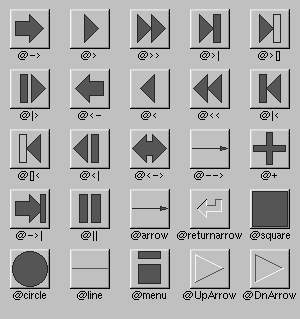
\includegraphics[scale=1]{symbols} 


 FLTK label supported symbols.


  The @ sign may be followed by the following optional ``formatting'' characters, in this order: 


 
\begin{enumerate}
\item 

 ``\#'' forces square scaling rather than distortion to the widget's shape.

\item 

 +[1-9] or -[1-9] tweaks the scaling a little bigger or smaller.

\item 

 [1-9] rotates by a multiple of 45 degrees. ``6'' does nothing, the others point in the direction of that key on a numeric keypad.


\end{enumerate}


 \emph{ion}
 -- value output when the button is checked. 


 \emph{ioff}
 -- value output when the button is unchecked. 


 \emph{itype}
 -- an integer number denoting the appearance of the widget. 


  Several kind of buttons are possible, according to the value of \emph{itype}
 argument: 


 
\begin{itemize}
\item 

 1 - normal button

\item 

 2 - light button

\item 

 3 - check button

\item 

 4 - round button


\end{itemize}


  This is the appearance of the buttons: 


 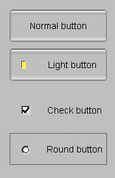
\includegraphics[scale=1]{flbutton} 


 FLbutton.


 \emph{iwidth}
 -- width of widget. 


 \emph{iheight}
 -- height of widget. 


 \emph{ix}
 -- horizontal position of upper left corner of the valuator, relative to the upper left corner of corresponding window (expressed in pixels). 


 \emph{iy}
 -- vertical position of upper left corner of the valuator, relative to the upper left corner of corresponding window (expressed in pixels). 


 \emph{iopcode}
 -- score opcode type. You have to provide the ascii code of the letter corresponding to the score opcode. At present time only ``i'' (ascii code 105) score statements are supported. A zero value refers to a default value of ``i''. So both 0 and 105 activates the \emph{i}
 opcode. A value of -1 disables this opcode feature. 
\subsection*{Performance}


 \emph{kout}
 -- output value 


 \emph{kp1}
, \emph{kp2}
, ..., \emph{kpN}
 -- arguments of the activated instruments. 


  Buttons of type 2, 3, and 4 also output (\emph{kout}
 argument) the value contained in the \emph{ion}
 argument when checked, and that contained in \emph{ioff}
 argument when unchecked. 


  By adding 10 to \emph{itype}
 argument (i.e. by setting 11 for type 1, 12 for type 2, 13 for type 3 and 14 for type 4) it is possible to skip the button value when getting/setting snapshots (see later section). \emph{FLbutton}
 not only outputs a value, but can also activate (or schedule) an instrument provided by the user each time a button is pressed. 


  If the \emph{iopcode}
 argument is set to a negative number, no instrument is activated. So this feature is optional. In order to activate an instrument, \emph{iopcode}
 must be set to 0 or to 105 (the ascii code of character ``i'', referring to the \emph{i}
 score opcode). 


  P-fields of the activated instrument are \emph{kp1}
 (instrument number), \emph{kp2}
 (action time), \emph{kp3}
 (duration) and so on with user p-fields. Notice that in dual state buttons (light button, check button and round button), the instrument is activated only when button state changes from unchecked to checked (not when passing from checked to unchecked). 
\subsection*{Examples}


  Here is an example of the flbutton opcode. It uses the files \emph{flbutton.orc}
, \emph{flbutton.sco}
, and \emph{beats.wav}
. 


 \textbf{Example 1. Example of the flbutton opcode.}

\begin{lstlisting}
/* flbutton.orc */
; Using fl-buttons to create on screen controls for play, 
; stop, fast forward and fast rewind of a sound file
; This example also makes use of a preset graphic for buttons.
sr = 44100
kr = 44100
ksmps = 1
nchnls = 1

FLpanel "Buttons", 320, 120, 100, 100
    ion = 0
    ioff = 0
    itype = 1
    iwidth = 50
    iheight = 50
    ix = 50
    iy = 35
    iopcode = 0
    istarttim = 0
    idur = -1

    ; Normal speed forwards
    gkplay, ihb1 FLbutton "@>", ion, ioff, itype, iwidth, iheight, ix, iy, iopcode, 1, istarttim, idur, 1 
    ; Stationary 
    gkstop, ihb2 FLbutton "@square", ion,ioff, itype, iwidth, iheight, ix+55, iy, iopcode, 1, istarttim, idur, 0
    ; Double speed backwards
    gkrew, ihb2 FLbutton "@<<", ion, ioff, itype, iwidth, iheight, ix+110, iy, iopcode, 1, istarttim, idur, -2
    ; Double speed forwardS
    gkff, ihb2 FLbutton "@>>", ion, ioff, itype, iwidth, iheight, ix+165, iy, iopcode, 1, istarttim, idur, 2
FLpanelEnd
FLrun

; Ensure that only 1 instance of instr 1
; plays even if the play button is clicked repeatedly
insnum = 1
icount = 1
maxalloc insnum, icount

instr 1
    asig diskin "beats.wav", p4, 0, 1
    out asig
endin
/* flbutton.orc */
        
\end{lstlisting}
\begin{lstlisting}
/* flbutton.sco */
; A sine wave
f 1 0 131072 10 1

; Real-time performance for 1 hour.
f 0 3600
e
/* flbutton.sco */
        
\end{lstlisting}
\subsection*{See Also}


 \emph{FLbox}
, \emph{FLbutBank}
, \emph{FLprintk}
, \emph{FLprintk2}
, \emph{FLvalue}

\subsection*{Credits}


 Author: Gabriel Maldonado


 New in version 4.22


 Example written by Iain McCurdy, edited by Kevin Conder.
%\hline 


\begin{comment}
\begin{tabular}{lcr}
Previous &Home &Next \\
FLbutBank &Up &FLcolor

\end{tabular}


\end{document}
\end{comment}
